%Copyright (c) 2004 2005 2006 Atos Origin
%Permission is granted to copy, distribute and/or modify this
%document
%under the terms of the GNU Free Documentation License,
%      Version 1.2
%      or any later version published by the Free Software
%      Foundation;
%      with no Invariant Sections, no Front-Cover
%      Texts, and no Back-Cover
%      Texts.  A copy of the license is
%      included in the section entitled "GNU
%      Free Documentation License".
%
%$Id: general_process.tex,v 1.1 2006/02/16 17:36:15 goneri Exp $
\section{General process}
\subsection{Four steps}
The general process of QSOS is made up of several interdependent steps (figure~\ref{fig-process}).

\begin{figure}[h]
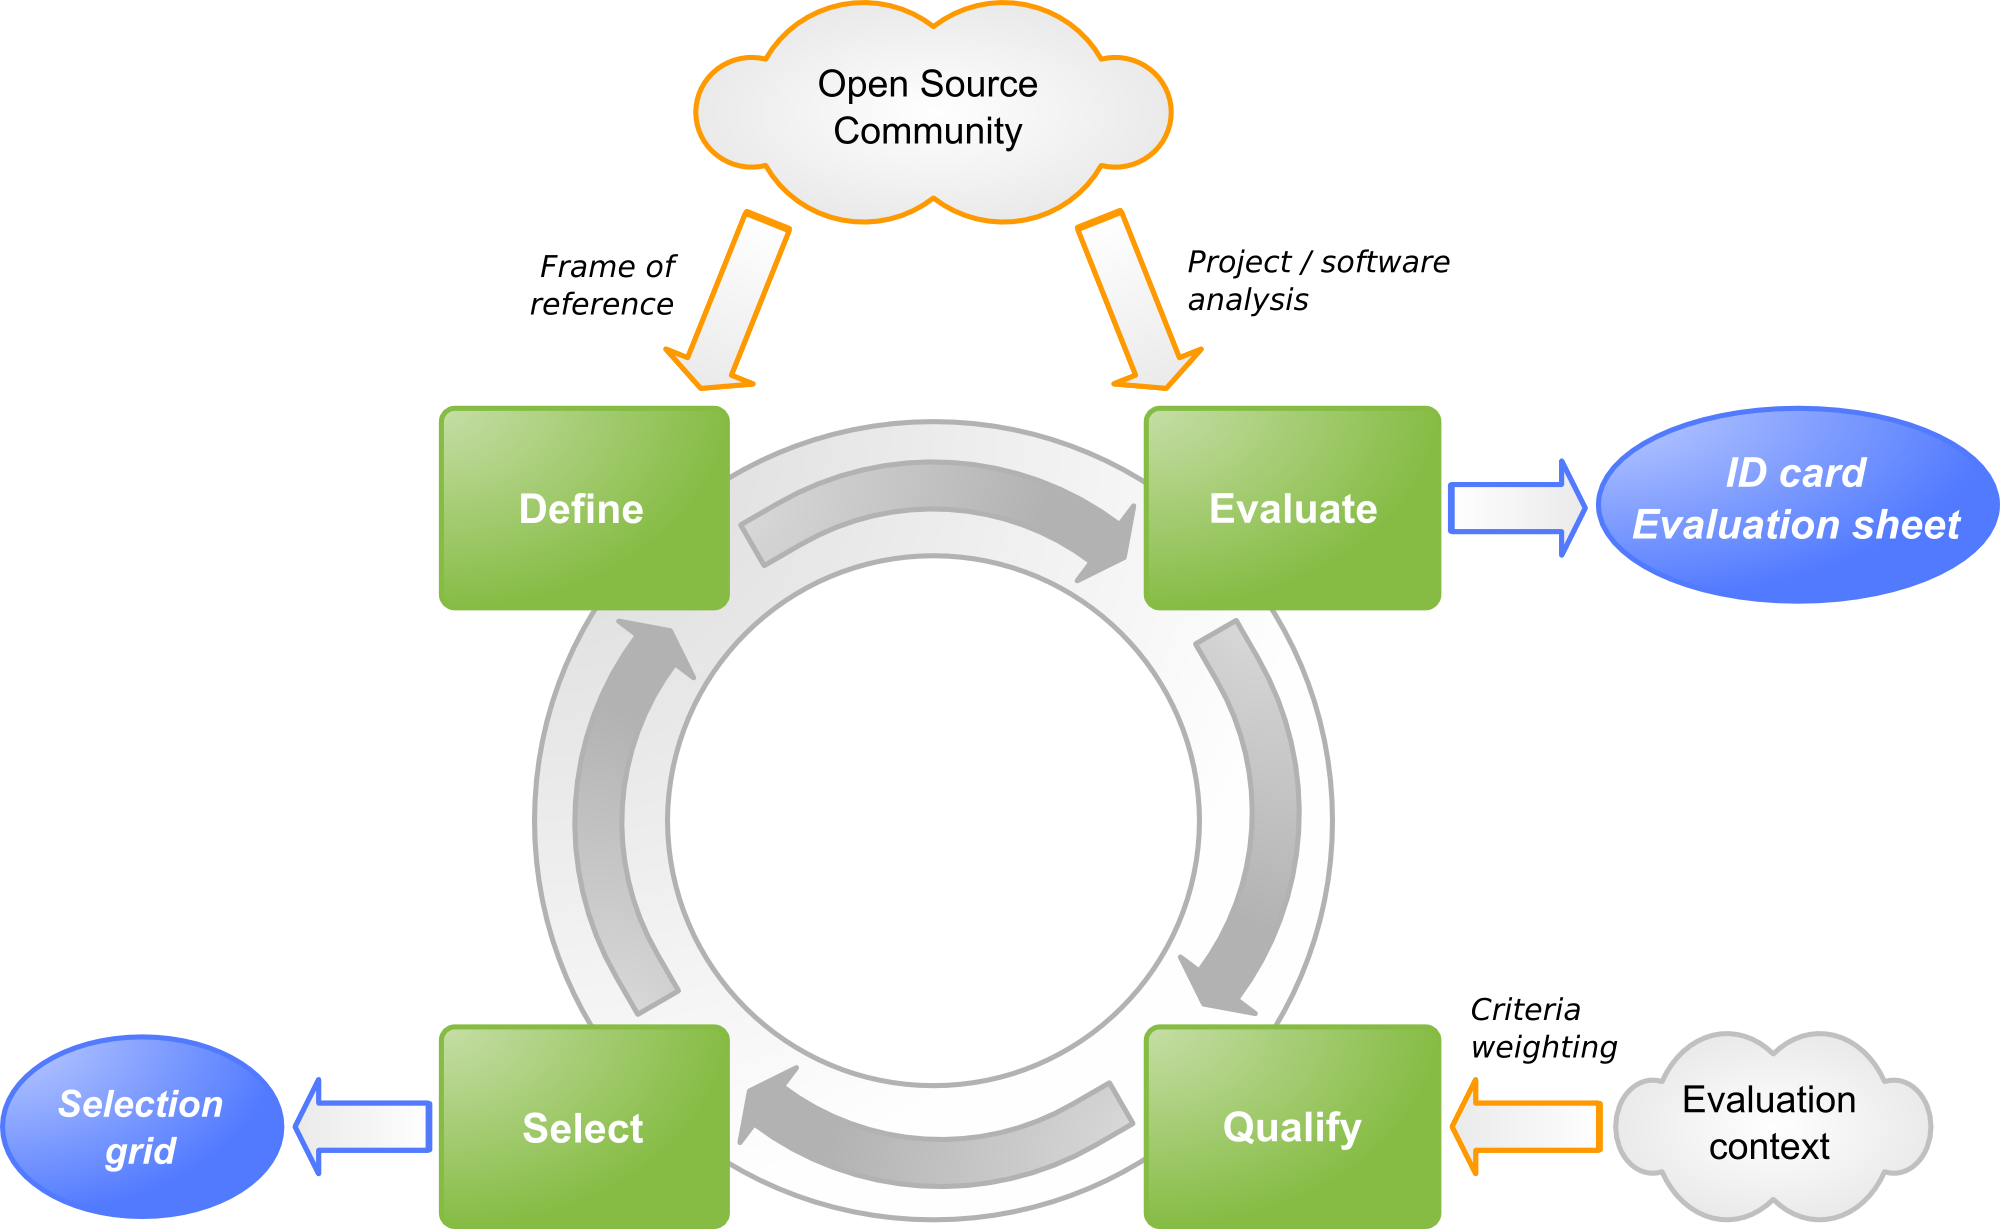
\includegraphics[width=16cm]{images/processus_4_etapes}
\caption{The 4 steps of QSOS}
\label{fig-process}
\end{figure}

\begin{figure}
%a faire en mieux
\center
\begin{tabular}{|p{3cm}|p{9cm}|}
\hline \TS{Step} & \TS{Description}\\
\hline 1 - Define & Constitution and enrichment of frames of reference used by following steps.\\
\hline 2 - Evaluate & Evaluation of software made on three axis of criteria: functional coverage, risks for the user and risks for the service provider (independently of any particular user/customer context).\\
\hline 3 - Qualify & Weighting of the criteria split up on the three axes, modeling the context (user requirements and/or strategy set by the service provider).\\
\hline 4 - Select & Application of the filter set up in Step 3 - "Qualify" on data provided by the first two steps, in order to proceed queries, comparisons and selections of products.\\
\hline
\end{tabular}
\end{figure}
Each one of these steps is detailed further in this document


\subsection{Iterative process}
The general process introduced here can be applied with different granularities. 
It allows to set the desired the level of detail for the process as well as to proceed by iterative 
loops to refine each of the four steps.


\subsection{Tools}
A single tool is being developped by Atos Origin to apply the QSOS method in a coherent way.

This tool, nammed O3S (Open Source Selection Software), will be made available to the community on the site \url{http://www.qsos.org} to coordinate creation, modification and use of QSOS evaluations.


